\section{Introduction}
The Whiley programming language has been in active development since
2009.  The language was designed specifically to help the programmer
eliminate bugs from his/her software.  The key feature is that Whiley
allows programmers to write {\em specifications} for their functions,
which are then checked by the compiler.  For example, here is the
specification for the \lstinline{max()} function which returns the
maximum of two integers:

\begin{lstlisting}
function max(int x, int y) => (int z)
// Must return either x or y
ensures x == z || y == z
// Return must be as large as x and y
ensures x <= z ${\tt \&\&}$ y <= z:
    ...
\end{lstlisting}
Here, we see our first piece of Whiley code.  This declares a function
called \lstinline{max} which accepts two integers \lstinline{x} and
\lstinline{y}, and returns an integer \lstinline{z}.  For now, we've
left out the body of this function and put ``\lstinline{...}'' in its
place.  The two \lstinline{requires} clauses form the function's {\em
  post-condition}, which is a guarantee made to any caller of this
function.  In this case, the \lstinline{max} function guarantees to
return one of the two parameters, and that the return will be as large
as both of them.  In plain English, this means it will return the
maximum of the two parameter values.  

When verification is enabled the Whiley compiler will check that every
function meets its specification.  For our \lstinline{max()} function,
this means it will check that body of the function guarantees to
return a value which meets the function's post-condition.  If not, the
compiler will report an error.  The advantage of supporting
specifications, is that they can help uncover bugs and other, more
serious, problems earlier in the development cycle.  This leads to
software which is both more reliable and more easily maintained (since
the specifications provide important documentation).

\subsection{Objectives}

Although the primary purpose of Whiley is to allow us to write
specifications on functions, we will not talk about that again until
the end of the document.  This goal of this article is to introduce
the core language without worrying too much about verification (since
this presents many challenges).  Indeed, it is only once we've
understood the basics of Whiley that we will will be ready to
investigate verification.

\subsection{Installation}

There are currently three ways to get setup with the Whiley
programming language:

\begin{itemize}
\item {\bf Web Browser.} By far the simplest way to get started with
  Whiley is by running it in your web browser (see
  Figure~\ref{whileyplay}).  Go to \url{http://whiley.org/play/} and
  you can get started straight away!
\item {\bf Eclipse Plugin.} If you're familiar with the Eclipse IDE or
  want to develop more serious programs in Whiley, then installing the
  Eclipse plugin is easy to do.  From within Eclipse, choose {\em
    Help$\rightarrow$Install New Software} from the menu.  Enter
  \url{http://whiley.org/eclipse} as the site, select the ``Whiley
  Eclipse Plugin'' and follow the on-screen instructions (see Figure~\ref{wyclipseinstall}).
\item {\bf Development Kit.} For those familiar with the command-line,
  installing the Whiley Development Kit (WDK) is another option.
  Furthermore, you'll be able to explore the source code for the
  Whiley system, and see how it all works!  To do this, visit
  \url{http://whiley.org/downloads/}.
\end{itemize}

More information of getting started with Whiley can be found at
\url{http://whiley.org/getting-started/}.  Finally, the Whiley system
is completely free and released under an open source license (BSD),
and you can get the latest code from \url{http://github.com/Whiley}.

\begin{figure}[!t]
\centering
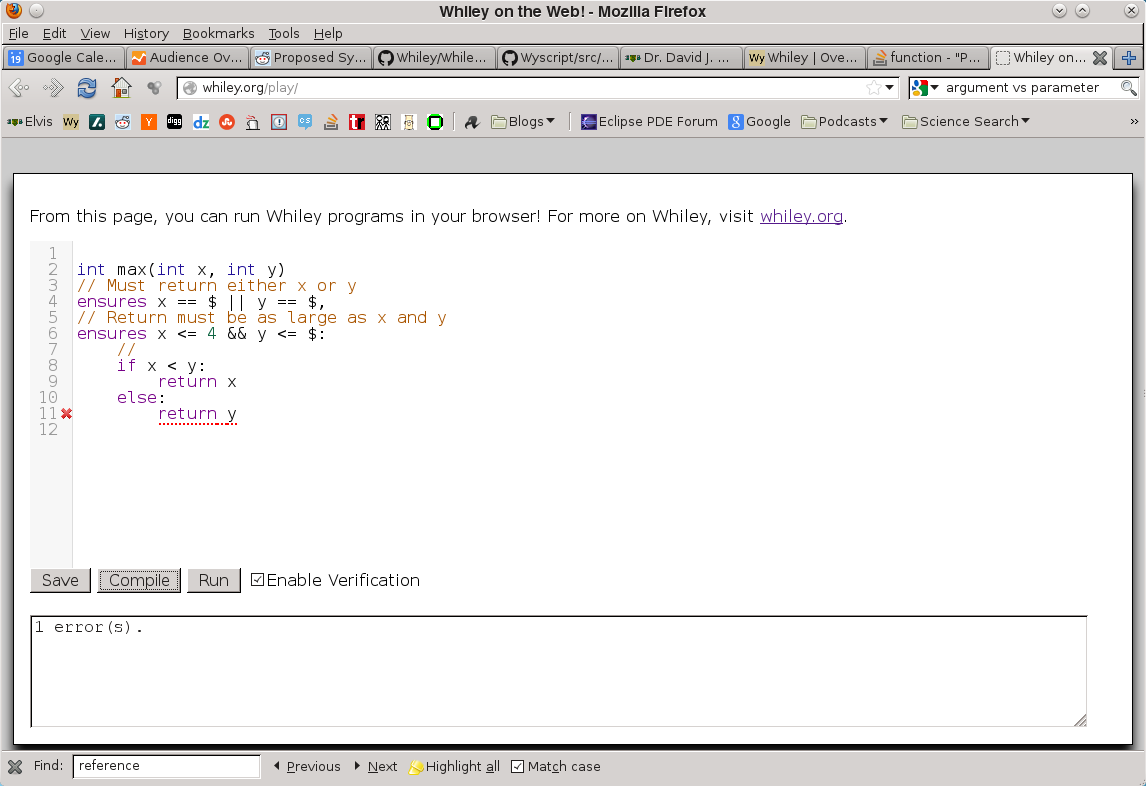
\includegraphics[width=0.9\textwidth]{../images/WhileyPlay.png}
\caption{Compiling a Whiley program using a web browser (Mozilla
  Firefox).  At the moment, the user's program is not correct since
  the system is reporting an error in red.}
\label{whileyplay}
\end{figure}

\begin{figure}[!t]
\centering
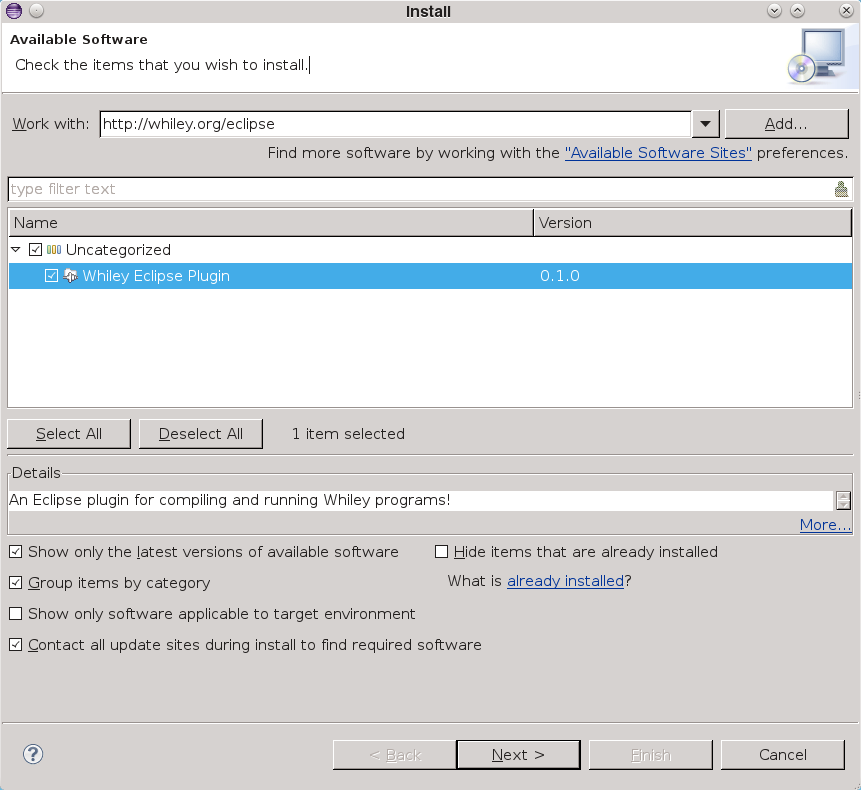
\includegraphics[width=0.9\textwidth]{../images/WyclipseInstallation.png}
\caption{Installing the Whiley Eclipse Plugin from within Eclipse.}
\label{wyclipseinstall}
\end{figure}

\clearpage
